\chapter{Functional Verification of Sequential Normal Basis Multiplier}
\label{ch:normal}
In order to utilize our traversal algorithm, it is necessary to find out
a sort of suitable circuit benchmarks which is easy to compute its
Gr\"bner basis (GB). From the work of Lv et al. \cite{lv_dissertation},
we learn that arithmetic circuits in Galois field (GF) is
convertible to an ideal of circuit polynomials, and the 
ideal generators form a GB themselves when applying reverse topological
term order. Furthermore, according to the work of Pruss et al.
\cite{tim_dissertation}, with a limited computation complexity,
we can abstract the word-level signature of an arithmetic 
component working in GF. Thus, we consider the possibility 
of applying our traversal algorithm on sequential Galois
field circuits. In each frame, we can use the techniques 
from \cite{tim_dissertation} to abstract the word-level
signature of the combinational logic, which corresponds
to the transition function in our traversal algorithm.
As a result, we manage to find a type of sequential GF multiplier
which we can apply our traversal algorithm to actually 
verify its functional correctness.

\section{Motivation}
\label{sec:normal_motiv}
From the preliminaries (Chapter \ref{ch:prelim}) about FSMs, we learn that the
Moore machine does not rely on inputs for state transitions. 
As depicted in Figure \ref{fig:Moore}(a), a typical Moore machine implementation
consists of combinational logic component and register files, where
$r_0,\dots,r_k$ are present state (PS) variables 
standing for state inputs (SI), and $r_0',\dots,r_k'$ are next state (NS) variables standing for
state outputs (SO). Figure \ref{fig:Moore}(b) shows the state transition graph (STG) of 
a Moore machine with $k+1$ distinct states. We notice that it forms a simple chain,
with $k$ consecutive transitions the machine reaches final state $R_k$.

\begin{figure}[H]
\centering{
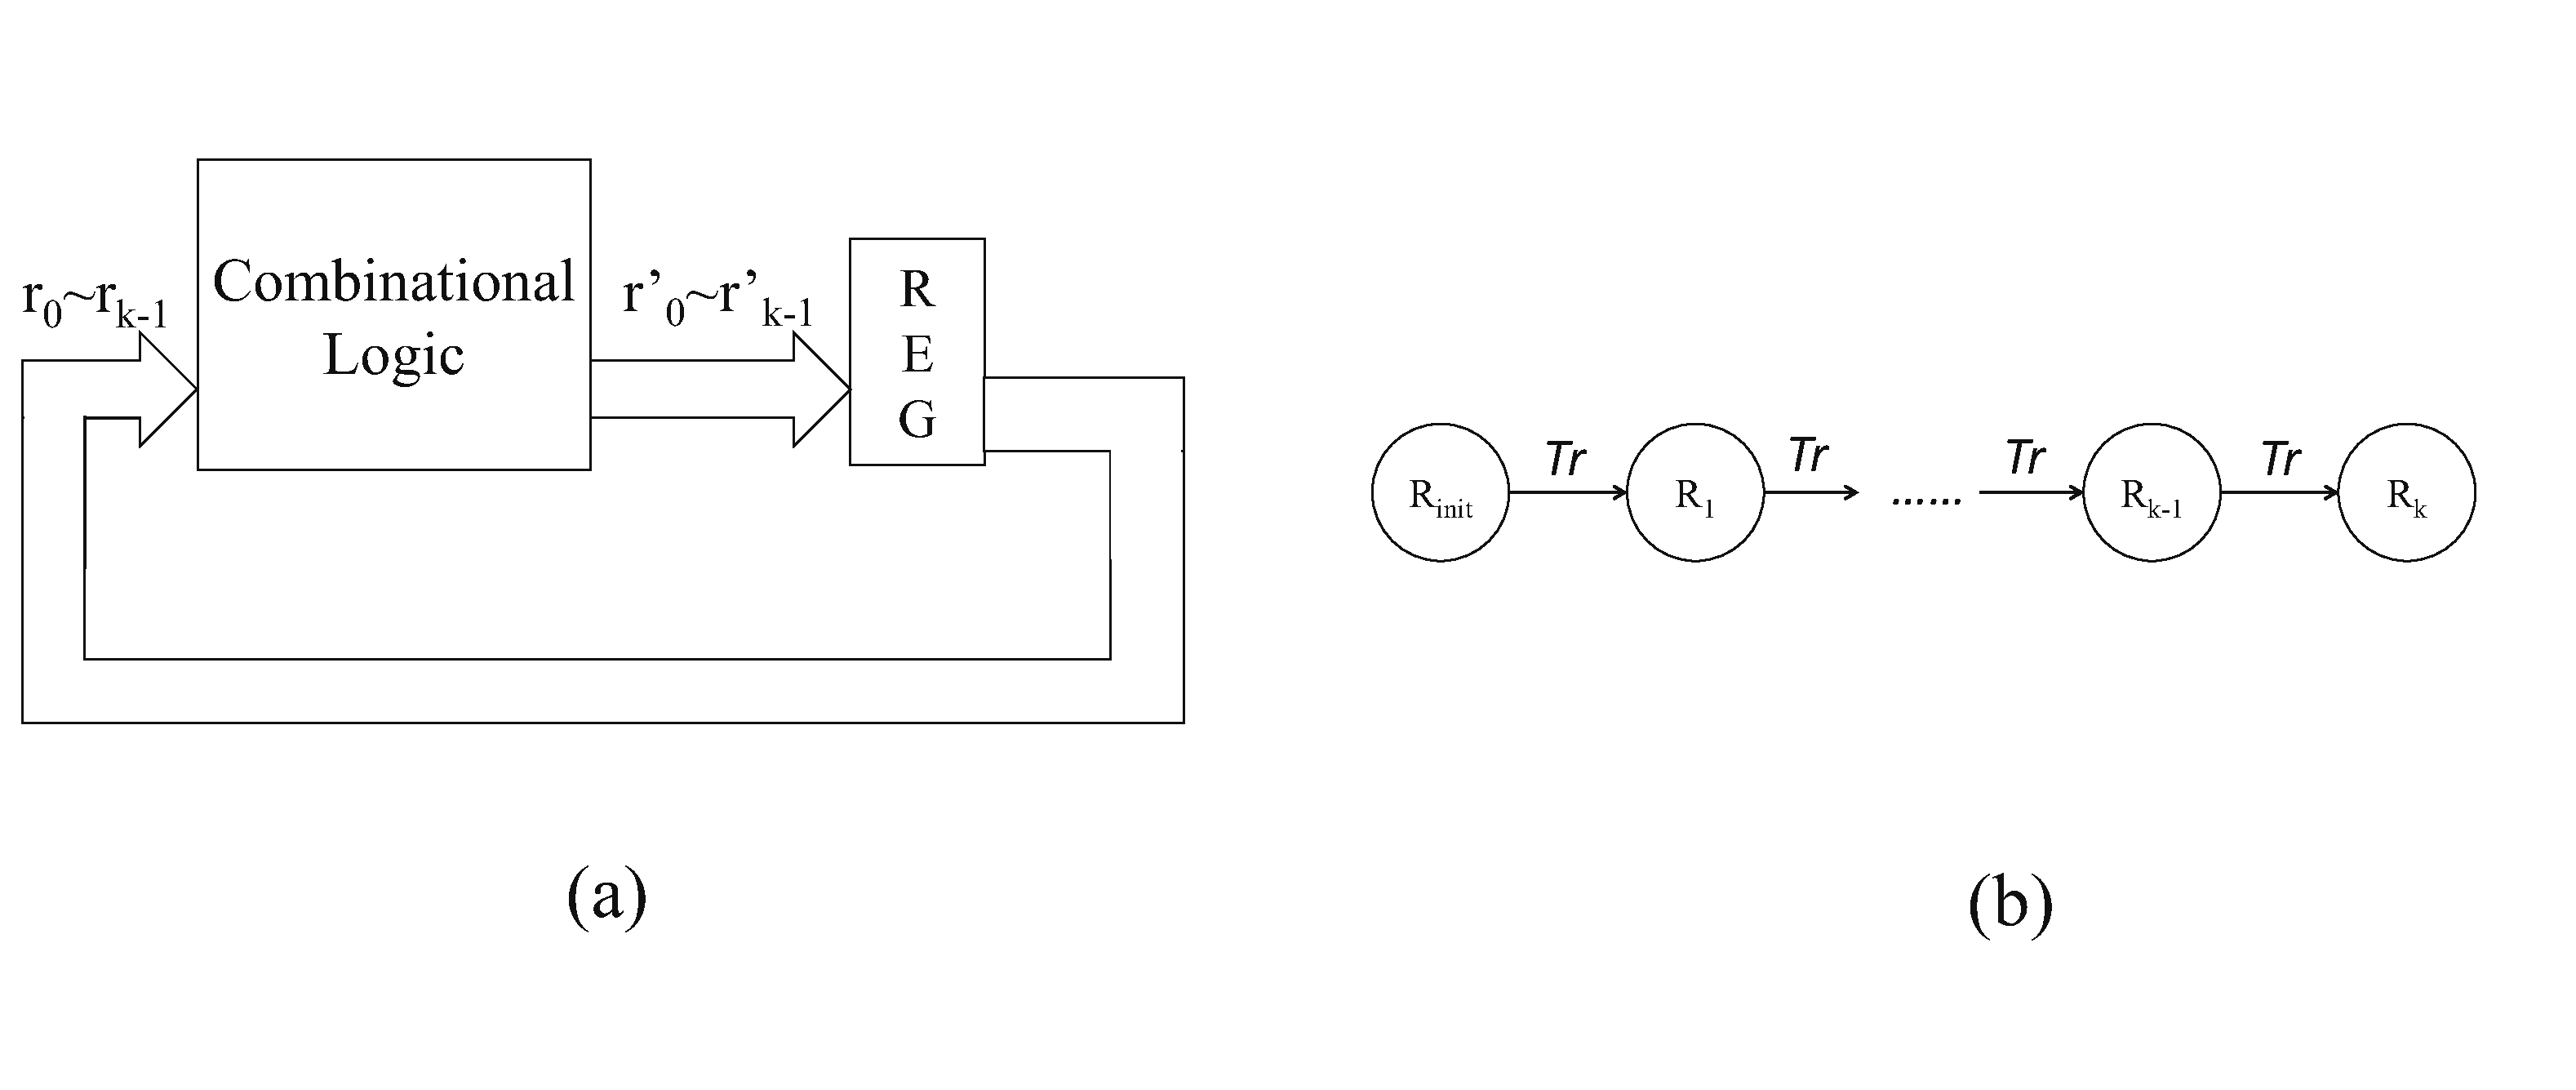
\includegraphics[width=3.5in]{newfig/Moore.eps}
\caption{A typical Moore machine and its state transition graph}
\label{fig:Moore}}
\end{figure}

In practice,
some arithmetic components are designed in sequential circuits similar to the structure in 
Figure \ref{fig:Moore}(a). Initially the operands are loaded into the registers, 
then the closed circuit executes without taking any additional information from outside,
and store the results in registers after $k$ clock cycles. Its behavior can be described using
STG in Figure \ref{fig:Moore}(b): state $R$ denotes the bits stored in registers. Concretely, $R_init$ is the initial
state (usually reset to all zeros), $R_1$ to $R_{k-1}$ are intermediate results stored as SO of current state and SI
for next state, and $R_k$ (or $R_{final}$) is the final result given by arithmetic circuits (and equals to the answer
to arithmetic function when circuit is working functional correctly).
This kind of design results in 
reusing a smaller combinational logic component such that the area cost is greatly optimized.
However, it also brings difficulties in verifying the the circuit functions.

\begin{figure}[H]
\centering{
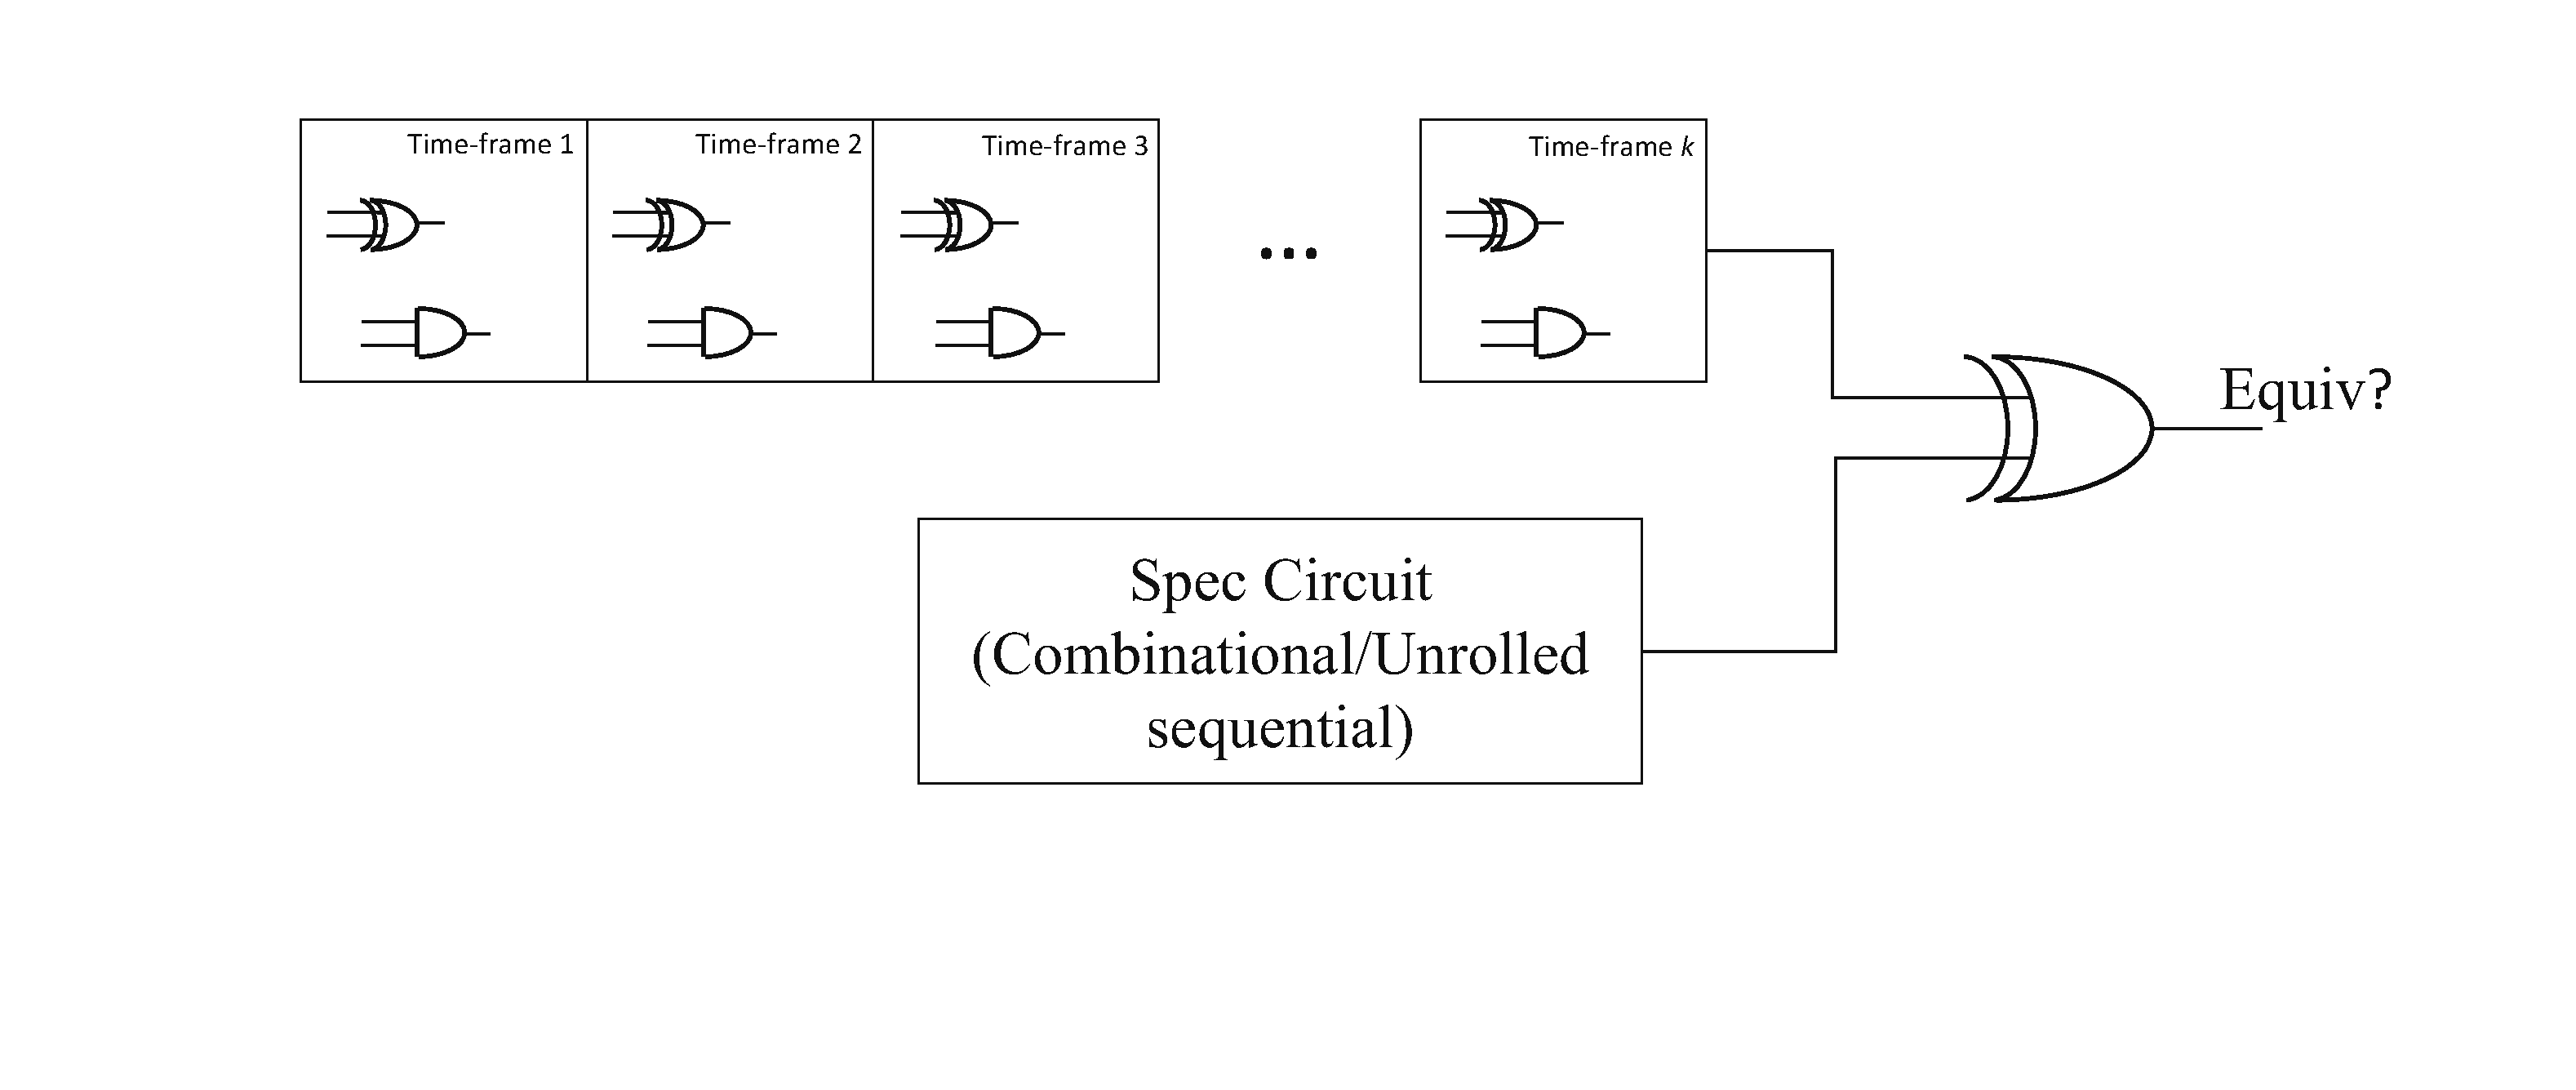
\includegraphics[width=3.5in]{newfig/convention.eps}
\caption{Conventional verification techniques based on bit-level unrolling and equivalence checking}
\label{fig:convention}}
\end{figure}

Conventional methods to such a sequential circuit may consist of unrolling the circuit for 
$k$ time-frames, and performing an equivalence checking between the unrolled machine and
the specification function. However, the number of gates will grow fast when doing unrolling
on bit-level. Meanwhile the structural similarity based equivalence checking techniques 
will fail when the sequential circuit is highly customized and optimized from the naive specification 
function. As a result, conventional techniques is grossly inefficient for large circuits.
Therefore, a new method based on our proposed word-level FSM traversal technique is worthy to be explored.

\section{Normal Basis Multiplier over Galois Field}
Given a Galois field (GF) $\Fkk$ is a finite field with  $2^k$ elements and characteristic equals to 2.
Its elements can be written in polynomials of $\alpha$, when there is an irreducible polynomial $p(\alpha)$
defined.

If we use a basis $(1,\alpha,\alpha^2,\alpha^3,\dots,\alpha^{k-1})$, we can easily transform polynomial representations
to binary bit-vector representations by recording the coefficients. For example,

\begin{table}[H]
\centering
\caption{Bit-vector, Exponential and Polynomial representation of
elements in  ${\mathbb{F}}_{2^4} = {\mathbb{F}}_2[x]
\pmod{x^4+x^3+1}$}
\begin{tabular}{|c|c||c|c|} 
\hline
$a_3a_2a_1a_0$ & Polynomial     &$a_3a_2a_1a_0$ & Polynomial  \\
\hline
$0000$        & $0$           & $1000$  &$\alpha^3$\\
\hline
$0001$        & $1$           & $1001$  & $\alpha^3 + 1$\\
\hline
$0010$        &  $\alpha$       & $1010$ & $\alpha^3 + \alpha$  \\
\hline
$0011$        &  $\alpha + 1$   & $1011$ &  $\alpha^3+\alpha+1$\\
\hline
$0100$        &  $\alpha^2$     &  $1100$ &  $\alpha^3 + \alpha^2$\\
\hline
$0101$        & $\alpha^2 + 1$ & $1101$  & $\alpha^3+\alpha^2+1$\\
\hline
$0110$        &  $\alpha^2 + \alpha$ & $1110$ &  $\alpha^3+\alpha^2+\alpha$\\
\hline
$0111$        & $\alpha^2+\alpha+1$ & $1111$ & $\alpha^3+\alpha^2+\alpha+1$\\
\hline
\end{tabular}
\label{table:booltogalois}  
\end{table}

Basis $(1,\alpha,\alpha^2,\alpha^3,\dots,\alpha^{k-1})$ is called {\bf standard basis} (StB), which results in
a straightforward representation for elements, and operations of elements such as addition and subtraction.
The addition/subtraction of GF elements in StB follows the rules of polynomial addition/subtraction
where coefficients belong to $\mathbb F_2$. In other words, using the definition of {\it exclusive or} in
Boolean algebra, element $A$ add/subtract by element $B$ in StB is defined as
\begin{align}
A+B = A-B &= (a_0,a_1,\dots,a_{k-1}) \xor (b_0,b_1,\dots,b_{k-1}) \nonumber\\
&=(a_0\oplus b_0, a_1\oplus b_1,\dots,a_{k-1}\oplus b_{k-1}) 
\end{align}